\begin{frame}
    \frametitle{Queues - Examples}
    \centering

    \tikzset{man/.pic={
        \node[circle, fill, minimum size=5mm] (head) {};
        \node[rounded corners = 2pt, minimum height = 0.8cm, minimum width=0.4cm,
            fill, below = 1pt of head] (body) {};
        \draw[line width = 1mm, round cap-round cap] 
            ([shift={(2pt,-1pt)}]body.north east) --++ (-90:6mm);
        \draw[line width=1mm,round cap-round cap] 
            ([shift={(-2pt,-1pt)}]body.north west) --++ (-90:6mm);
        \draw[line width = 2mm, round cap-round cap] 
            ([shift={(-3.3pt,3.7pt)}]body.south east) --++ (-83:6mm);
       \draw[line width = 2mm, round cap-round cap] 
            ([shift={(3.3pt,3.7pt)}]body.south west) --++ (-97:6mm);
    }}


    \only<1>{
        \scalebox{0.8}{
            \begin{tikzpicture} 
                \foreach \j in {1,...,5}
                    \pic[orange] at (\j*1.5 - 1, 0) {man};
                \pic[orange] at (9, 0) {man};
                \draw[fill = orange] (8, -0.5) rectangle (10, -1.6);
            \end{tikzpicture}
        }
        \vspace{4cm}
    }
    \only<2>{
        \scalebox{0.8}{
            \begin{tikzpicture} 
                \foreach \j in {1,...,5}
                    \pic[orange] at (\j*1.5 - 1, 0) {man};
                \pic[orange] at (9, 0) {man};
                \draw[fill = orange] (8, -0.5) rectangle (10, -1.6);
            \end{tikzpicture}
        }
        \footnotesize
        \vspace{1cm}
        \begin{itemize}
            \item Shone R, Knight VA, Williams JE. Comparisons between observable and unobservable M/M/1 queues with respect to optimal customer behaviour
            \item Kerner Y, Shmuel-Bittner O. Strategic behaviour and optimization in a hybrid M/M/1 queue with retrials.
            \item Gai Y, Liu H, Krishnamachari B. A packet dropping mechanism for efficient operation of M/M/1 queues with selfish users.
        \end{itemize}
    }

    \only<3>{
        \scalebox{0.8}{
            \begin{tikzpicture}
                \foreach \i in {1,...,5}
                \pic[cyan] at (\i*1.5 - 1, 0) {man};
                
                \foreach \j in {2, -0.5, -3}{
                    \pic[cyan] at (9, \j + 0.5) {man};
                    \draw[fill = cyan] (8, \j) rectangle (10, \j -1.1);
                }
            \end{tikzpicture}
        }
    }

    \only<4>{
        \scalebox{0.8}{
            \begin{tikzpicture}
                \foreach \i in {1,...,5}
                \pic[cyan] at (\i*1.5 - 1, 0) {man};
                
                \foreach \j in {2, -0.5, -3}{
                    \pic[cyan] at (9, \j + 0.5) {man};
                    \draw[fill = cyan] (8, \j) rectangle (10, \j -1.1);
                }
            \end{tikzpicture}
        }
        \footnotesize
        \vspace{0.5cm}
        \begin{itemize}
            \item Knight V, Harper P. The Impact of Choice on Public Services.
            \item Wang X, Song C, Zhuang J. Simulating a multi-stage screening network: A queueing theory and game theory application.
        \end{itemize}
    }


    \only<5>{
        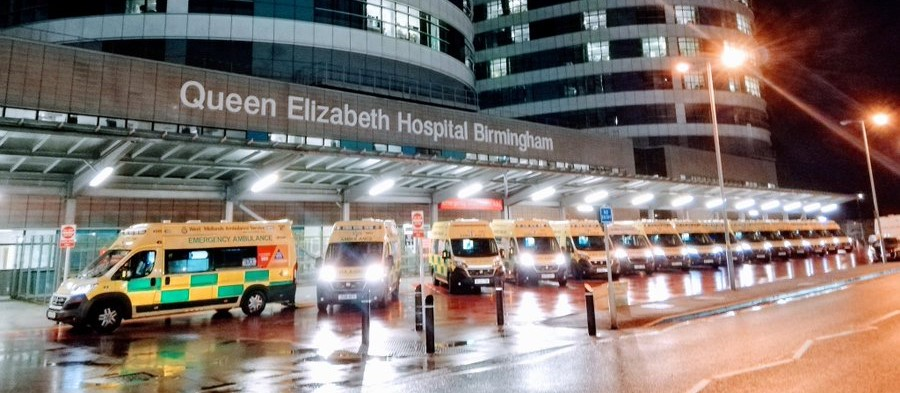
\includegraphics[scale=0.45]{Bin/ambulance_queue.jpg}
    }
\end{frame}